\columnbreak

\subsection{Examples}

\begin{example2}{Load/Store Architecture}
What is a load/store architecture?
\begin{itemize}
  \item Data processing is between registers
  \item Transfer of data from and to the external memory is done using load (memory to register) or store (register to memory) instructions
\end{itemize}
\end{example2}

\begin{example2}{MOV vs MOVS Instructions}\\
Key differences between MOV and MOVS:
\begin{itemize}
  \item \textbf{MOV}: Transfer does NOT affect flags (low and high registers)
  \item \textbf{MOVS}: Transfer affects flags (only low registers)
\end{itemize}
\end{example2}



\begin{example2}{Initializing Registers}\\
Different ways to initialize a register with immediate value:

1. Using MOVS:
\begin{lstlisting}[language=armasm, style=basesmol]
MOVS    R0, #42         ; Limited to 8-bit values
\end{lstlisting}
Advantages:
\begin{itemize}
  \item Value is in instruction
  \item Less memory space needed
\end{itemize}
Disadvantages:
\begin{itemize}
  \item Limited to 8-bit values
  \item Only works with low registers
\end{itemize}

2. Using LDR with PC-relative addressing:
\begin{lstlisting}[language=armasm, style=basesmol]
LDR     R0, [PC, #12]   ; Can load 32-bit values
\end{lstlisting}
Advantages:
\begin{itemize}
  \item Can load larger values (up to 32-bit)
  \item Works with any register
\end{itemize}
Disadvantages:
\begin{itemize}
  \item Takes more space in memory
  \item Requires literal pool management
\end{itemize}
\end{example2}

\begin{example2}{Data transfer instruction for high registers}\\
Which data transfer instructions should you use if at least one high register is an operand?\\
MOV works for all registers (but only for reg/reg transfers)
\end{example2}

\begin{example2}{Initializing low registers}\\
List different ways of initializing a low register with an immediate value. What are the advantages/disadvantages?
\vspace{2mm}\\
\texttt{MOVS <Rd>,\#<imm8>}\\
Value to load is in instruction\\
Less memory space but limited to 8-bit values.
\vspace{2mm}\\
\texttt{LDR <Rt>, [PC,\#<imm>]}\\
Use PC/offset combination to point to the value to load.\\
Can be used to load larger values (up to 32 -bit). Takes more space in memory.
\end{example2}



\begin{KR}{Register Transfer Operations}\\
Steps for data transfer operations:

1. Moving between registers:
\begin{lstlisting}[language=armasm, style=basesmol]
; Copy contents with flags unchanged
MOV     R3, R1          ; For any registers

; Copy contents and update flags
MOVS    R3, R1          ; Only for low registers
\end{lstlisting}

2. Loading immediate values:
\begin{lstlisting}[language=armasm, style=basesmol]
; Small values (flags unchanged)
MOV     R0, #42         ; 8-bit immediate

; Larger values
LDR     R0, =0x12345678 ; 32-bit value using literal pool

; For high registers
LDR     R0, =value      ; Load into low register first
MOV     R8, R0          ; Then move to high register
\end{lstlisting}

3. Memory access:
\begin{lstlisting}[language=armasm, style=basesmol]
; Load from memory
LDR     R0, [R1]        ; Word from address in R1
LDRB    R0, [R1]        ; Byte from address in R1

; Store to memory
STR     R0, [R1]        ; Word to address in R1
STRB    R0, [R1]        ; Byte to address in R1
\end{lstlisting}
\end{KR}

\begin{example2}{Assembly Instructions for Memory Access}\\
Write down the assembly instructions to perform the following actions
\begin{itemize}
  \item Copy contents of R1 in R3 (flags unchanged)\\
  \texttt{MOV R3, R1}
  \item Initialize RO with $0 \times A A$ (flags unchanged)\\
  \texttt{LDR R0,=0xAA}
  \item Initialize R1 with 234 (flags modified)\\
  \texttt{MOVS R1,\#234}
  \item Initialize R4 with $0 \times 55 \mathrm{AACC}$\\
  \texttt{LDR R4,=0x55AACC}
  \item Copy contents of R9 in R3\\
  \texttt{MOV R3, R9}
  \item Initialize R10 with $0 \times 345678$\\
  \texttt{LDR R0,=0x345678 ; R0} as example. \\Another low register is ok:
  \texttt{MOV R10, R0}
  \item Copy contents of R8 in R9\\
  \texttt{MOV R9, R8}
\end{itemize}
\end{example2}



\begin{KR}{Array Access}\\
Guidelines for working with arrays:

1. Calculate element offset:
\begin{itemize}
  \item Byte arrays: offset = index
  \item Half-word arrays: offset = index × 2
  \item Word arrays: offset = index × 4
\end{itemize}

2. Choose appropriate instructions:
\begin{lstlisting}[language=armasm, style=basesmol]
    ; Array base in R0, index in R1
    
    ; For byte array
    LDRB    R2, [R0, R1]    ; index offset
    
    ; For half-word array
    LSLS    R2, R1, #1      ; multiply index by 2
    LDRH    R3, [R0, R2]    ; load half-word
    
    ; For word array
    LSLS    R2, R1, #2      ; multiply index by 4
    LDR     R3, [R0, R2]    ; load word
\end{lstlisting}

3. Consider alignment:
\begin{itemize}
  \item Words must be aligned to 4-byte boundary
  \item Half-words must be aligned to 2-byte boundary
  \item Bytes have no alignment requirement
\end{itemize}
\end{KR}

\begin{remark}
Important considerations:
\begin{itemize}
  \item Always check alignment requirements
  \item Be aware of endianness (STM32 is little-endian)
  \item Consider using multiple register transfer for efficiency
  \item Manage literal pool placement carefully
  \item Stack operations must maintain SP word alignment
\end{itemize}
\end{remark}


\begin{example2}{Pseudo-Instructions}\\
What is a pseudo-Instruction? \\Explain what is done with a <LDR Rn, =literal> pseudo-instruction.
\vspace{2mm}\\
A pseudo-Instruction does not directly translate in machine code. It is an instruction that is interpreted (or expanded)by the assembler (the tool) to generate the needed machine code instruction(s).
\vspace{2mm}\\
When we run the assembler (the tool), the <LDR Rn, =literal> instruction is decomposed into a place reservation of the type DCD and an indirect load of the type LDR <Rt>,[PC,\#<imm>] to get the contents of the reserved position and write it in Rn
\vspace{2mm}\\
Literal can be an address (a position in the memory)\\
Literal can be a constant (the value is known at assembling time)
\end{example2}



\begin{example2}{Register Content and Memory Positions}\\
Whenever possible, work out the contents of registers or memory positions that have changed.

\begin{center}
\begin{tabular}{|c|c|c|c|}
\hline
again & LDR & R0, $=0 \times F F$ & \textcolor{darkred}{R0 = 0x000000FF} \\
\hline
 & LDR & R1, lit1 & \textcolor{darkred}{R1 = 0x0000EFAA} \\
\hline
 & LDR & R2, lit2 & \textcolor{darkred}{R2 = 0x00012345} \\
\hline
 & LDR & R3, $=0 \times 55 \mathrm{AA}$ & \textcolor{darkred}{R3 = 0x000055AA} \\
\hline
 & MOV & R4, R1 & \textcolor{darkred}{R4 = 0x0000EFAA} \\
\hline
 & MOV & R4, R2 & \textcolor{darkred}{R4 = 0x00012345} \\
\hline
 & MOV & R6, R3 & \textcolor{darkred}{R6 = 0x000055AA} \\
\hline
 & MOVS & R7, \#04 & \textcolor{darkred}{R7 = 0x00000004} \\
\hline
 & LDR & R0, =lit1 & \begin{tabular}{l}
R0 = address of lit1 \\
(Address is not known) \\
\end{tabular} \\
\hline
 & LDR & R1, =lit2 & \textcolor{darkred}{R1 = address of lit2} \\
\hline
 & LDR & R2, =lit3 & \textcolor{darkred}{R2 = address of lit3} \\
\hline
 & LDRB & R5, [R2] & \textcolor{darkred}{R5 = 0x00000097} \\
\hline
 & LDRH & R6, [R2,\#2] & \textcolor{darkred}{R6 = 0x0000008F} \\
\hline
 & LDR & R2, [R0] & \textcolor{darkred}{R2 = 0x0000EFAA} \\
\hline
 & LDR & R3, [R0, \#4] & \textcolor{darkred}{R3 = 0x00012345} \\
\hline
 & STR & R3, [R1] & \textcolor{darkred}{lit2 = 0x00012345} \\
\hline
 & STR & R2, [R1, \#8] & \textcolor{darkred}{lit4 = 0x0000EFAA} \\
\hline
 & STR & R4, [R1, R7] & \textcolor{darkred}{lit3 = 0x00012345}  \\
 & & & (writes to  \\
 & & & (address of lit2 + R7)) \\
\hline
 & LDR & R5, =lit5 & \textcolor{darkred}{R5 = address of lit5} \\
\hline
 & MOVS & R0, \#0 & \textcolor{darkred}{R0 = 0x00000000} \\
\hline
 & ADDS & R7, R0, \#1 & \textcolor{darkred}{R7 = 0x00000001} \\
\hline
 & LDRSB & R6, [R5, R0] & \textcolor{darkred}{R6 = 0xFFFFFF89} \\
\hline
 & LDRSH & R6, [R5, R7] & \textcolor{darkred}{Problem: Unaligned}  \\
 & & & memory access \\
\hline
 & B & Again &  \\
\hline
lit1 & DCD & 0xEFAA &  \\
\hline
lit2 & DCD & 0x12345 &  \\
\hline
lit3 & DCD & 0x8F1097 &  \\
\hline
lit4 & DCD & 0xFF76552F &  \\
\hline
lit5 & DCD & 0xAA654389 &  \\
\hline
lit6 & DCD & 0x0165 &  \\
\hline
Var1 & DCD & 0x23 &  \\
\hline
Var2 & DCD & 0x24 &  \\
\hline
Var3 & DCD & $0 \times 23455678$ &  \\
\hline
Var4 & DCD & 0xE4568900 &  \\
\hline
\end{tabular}
\end{center}
\end{example2}

\begin{example2}{Assembled Listings}\\
\textcolor{pink}{\textbf{see exercise 8 in exercise sheet 3 - Data Transfer Instructions}}
this is way too much text for this summary
\end{example2}

\textcolor{pink}{\textbf{TODO: Add more examples}} and understand exercises from exercise sheet 3... help

\begin{example2}{Handling Pointers}\\
Example C code and assembly implementation:
\begin{lstlisting}[language=C, style=basesmol]
uint32_t x;
uint32_t y;
uint32_t *xp;

void main(void) {
    x = 3;
    xp = &x;
    y = *xp;
}
\end{lstlisting}

Assembly implementation:
\begin{lstlisting}[language=armasm, style=basesmol]
    AREA    myVar, DATA, READWRITE
X   DCD     0
Y   DCD     0
XP  DCD     0

    AREA    myCode, CODE, READONLY
main
    ; Get addresses
    LDR     R3, =X      ; Address of X
    LDR     R4, =Y      ; Address of Y
    LDR     R5, =XP     ; Address of XP
    
    ; x = 3
    MOVS    R0, #3      ; Load immediate value
    STR     R0, [R3]    ; Store in X
    
    ; xp = &x
    STR     R3, [R5]    ; Store address of X in XP
    
    ; y = *xp
    LDR     R2, [R5]    ; Load address from XP
    LDR     R1, [R2]    ; Load value from address
    STR     R1, [R4]    ; Store in Y
\end{lstlisting}
\end{example2}

\begin{comment}
9. In the following C program, code the statements in bold green in assembly.

\begin{verbatim}
// C-Code
uint32_t x;
uint32_t y;
uint32_t *xp;
void main(void) {
    x = 3;
    xp = &x;
    y = *xp;
}
\end{verbatim}

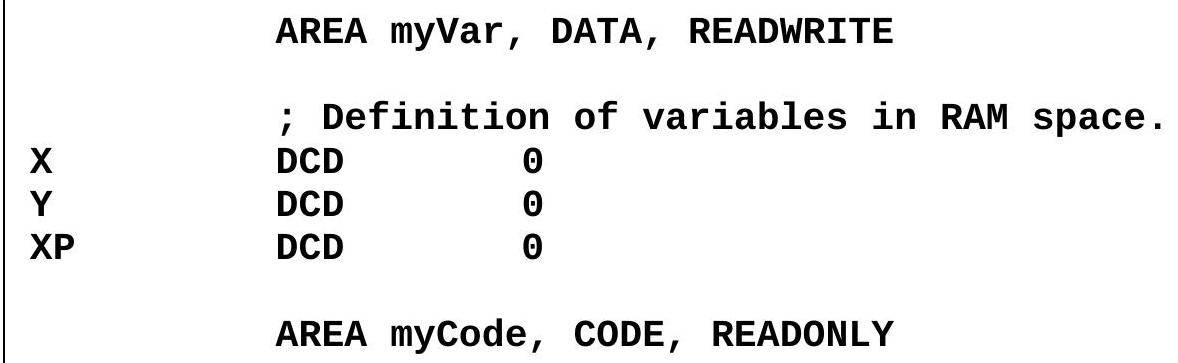
\includegraphics[width=\linewidth]{images/2025_01_02_eeffad754b73de6041b6g-05}\\
main

\begin{verbatim}
; This program is written in order to make it easy to understand
; Efficiency is not the important aspect in this implementation
; First point to variables using registers
LDR R3,=X ; initialize R3 with address of X
    ; reserve place to store address of X in literal pool
LDR R4,=Y ; initialize R4 with address of Y
    ; reserve place to store address of Y in literal pool
LDR R5,=XP ; initialize R5 with address of XP
    ; reserve place to store address of XP in literal pool
; X = 3
LDR R0,=0x03 ; load '3'
STR R0,[R3] ; and store it in X
;XP = &X
STR R3,[R5] ; store address of X (that address is in R3)
    ; in XP (address of XP is in R5)
;Y = *XP
LDR R2,[R5] ; read contents of XP variable (pointed to by
, R5) into R2. Address of X now in R2
LDR R1,[R2] ; read contents of X in R1
STR R1,[R4] ; store R1 (contents of X) in Y (pointed to by R4)
\end{verbatim}

\begin{enumerate}
  \setcounter{enumi}{9}
  \item In the following C program, code the statements in bold green in assembly. Use the frame for solution on following page.
\end{enumerate}

\begin{verbatim}
// C-Code
uint8_t demoArray[2];
uint8_t *xp;
void main(void) {
    demoArray[0] = 10;
    demoArray[1] = 11;
    xp = demoArray;
    *xp = 111;
    xp++;
    *xp = 112;
}
Note: Other statements of the C program are shown in frame with machine code and addresses as examples to help you.
You are only required to write the assembly code (not the machine code).
\end{verbatim}

Frame for solution

Possible solution, as given by the C compiler. This solution does not use pseudo instructions. Before looking at it, make sure that you understand the solution of 9a

22: demoArray[0] = 10;

\begin{center}
\begin{tabular}{|c|c|c|c|}
\hline
0x08000254 & 200A & MOVS & r0,\#0x0A \\
\hline
0x08000256 & 4909 & LDR & r1, [pc,\#36] \\
\hline
0x08000258 & 7008 & STRB & r0, [r1, \#0x00] \\
\hline
23: & \multicolumn{3}{|l|}{demoArray[1] = 11;} \\
\hline
0x0800025A & 200B & MOVS & r0,\#0x0B \\
\hline
0x0800025C & 7048 & STRB & r0, [r1, \#0x01] \\
\hline
\end{tabular}
\end{center}

\begin{center}
\begin{tabular}{|c|c|c|c|}
\hline
\multicolumn{4}{|l|}{24: $\quad \mathrm{xp}=$ demoArray;} \\
\hline
0x0800025E & 4608 & MOV & r0, r1 \\
\hline
0x08000260 & 4907 & LDR & r1, [pc,\#28] \\
\hline
0x08000262 & 6008 & STR & r0, [r1, \#0x00] \\
\hline
$25:$ & \multicolumn{3}{|l|}{${ }^{\text {xp }}$ = 111;} \\
\hline
0x08000264 & 206F & MOVS & r0,\#0x6F \\
\hline
0x08000266 & 6809 & LDR & r1, [r1, \#0x00] \\
\hline
0x08000268 & 7008 & STRB & r0, [r1, \#0x00] \\
\hline
$26:$ & \multicolumn{3}{|l|}{xp++;} \\
\hline
0x0800026A & 4805 & LDR & r0, [pc,\#20] \\
\hline
0x0800026C & 6800 & LDR & r0, [r0, \#0x00] \\
\hline
0x0800026E & 1C40 & ADDS & r0, r0, \#1 \\
\hline
0x08000270 & 4903 & LDR & r1, [pc,\#12] \\
\hline
0x08000272 & 6008 & STR & r0, [r1, \#0x00] \\
\hline
27 : & \multicolumn{3}{|l|}{*xp = 112;} \\
\hline
0x08000274 & 2070 & MOVS & r0,\#0x70 \\
\hline
0x08000276 & 6809 & LDR & r1, [r1, \#0x00] \\
\hline
0x08000278 & 7008 & STRB & r0, [r1, \#0x00] \\
\hline
\end{tabular}
\end{center}

28: \}\\
0x0800027A $4770 \quad$ BX $\quad$ lr ; Not part of solution\\
0x0800027C 0000 DCW 0x0000\\
0x0800027E 2000 DCW 0x2000\\
0x08000280 0004 DCW 0x0004\\
0x08000282 2000 DCW 0x2000\\
This correction shows opcode and assembly instruction to help you understand more. For the solution, only the assembly is required.\\
11. Consider the following listing.

\begin{verbatim}
\begin{tabular}{llll} 
080000008 4804 & again & LDR & R0, lit1 \\
0800000A 480A & & LDR & R0, =lit1 \\
0800000C 4A04 & & LDR & R2, lit2 \\
0800000E 4A0A & & LDR & R2, =lit2 \\
08000010 4B04 & & LDR & R3, lit3 \\
08000012 4C04 & & LDR & R4, lit3 \\
08000014 4E09 & R6, =lit4 \\
08000016 4F09 & & LDR & R7, =lit4 \\
08000018 4408 & & ADD & R0, R1 \\
0800001A E7F5 & B & again
\end{tabular}
0800001C 00000001
xxx DCD 0x01 ; xxx stands for a label
0 8 0 0 0 0 2 0 0 0 0 0 0 0 0 2
    xxx DCD 0x02
0 8 0 0 0 0 2 4 0 0 0 0 0 0 0 3
    xxx DCD 0x03
08000028 00000004
0800002C 00000005
0 8 0 0 0 0 3 0 0 0 0 0 0 0 0 6
08000034
    00000000
    00000000
    00000000
    00000000
\end{verbatim}

a) Compute on the basis of the opcode (marked in blue) the position where data is read to load registers (see table with example)

\begin{center}
\begin{tabular}{|l|l|l|l|}
\hline
\begin{tabular}{l}
Instruction \\
address \\
\end{tabular} & \begin{tabular}{l}
Opcode \\
(marked in blue) \\
\end{tabular} & \begin{tabular}{l}
position where \\
data is read \\
\end{tabular} & \begin{tabular}{l}
Contents of affected \\
register after operation \\
\end{tabular} \\
\hline
08000008 & 4804 & $0 \times 0800001 \mathrm{C}$ & $\mathrm{R0}=0 \times 00000001$ \\
\hline
 &  &  &  \\
\hline
 &  &  &  \\
\hline
 &  &  &  \\
\hline
 &  &  &  \\
\hline
 &  &  &  \\
\hline
 &  &  &  \\
\hline
\end{tabular}
\end{center}

b) The opcodes for <LDR R0, lit1> and <LDR R0, =lit1> are the same. But where are the operands? Explain the differences between the 2 .\\
c) Compute the contents of the registers after each instruction is executed once. Write results in table in a).

Example solutions will be written here

\begin{center}
\begin{tabular}{|l|l|l|l|}
\hline
\begin{tabular}{l}
Instruction \\
address \\
\end{tabular} & Opcode & \begin{tabular}{l}
position where \\
data is read \\
\end{tabular} & \begin{tabular}{l}
Contents of affected \\
register after operation \\
\end{tabular} \\
\hline
08000008 & 4804 & $0 \times 0800001 \mathrm{C}$ & R0 = 0x00000001 \\
\hline
0800000 A & 480A & $0 \times 08000034$ & R0 = 0x0800001C \\
\hline
0800000 C & 4A04 & $0 \times 08000020$ & R2 = 0x00000002 \\
\hline
0800000 E & 4A0A & $0 \times 08000038$ & R2 $=$ 0x08000020 \\
\hline
08000010 & 4B04 & $0 \times 08000024$ & R3 = 0x00000003 \\
\hline
08000012 & 4C04 & $0 \times 08000024$ & R4 = 0x00000003 \\
\hline
08000014 & 4E09 & $0 \times 0800003 C$ & R6 = 0x08000028 \\
\hline
08000016 & 4F09 & 0x0800003C & R7 = 0x08000028 \\
\hline
\end{tabular}
\end{center}

b) <LDR R0, lit1> The value at position label lit1 is loaded in R0\\
<LDR R0, =lit1> Of the form LDR r0, =label\\
(Room is made in the literal pool to store the address of lit1. That address is then loaded in R0 when code is executed)\\
<LDR R0, =const> (e.g. in previous exercise LDR R0, =0xFF55AAB0) Of the form LDR ro, = constant(The constant is placed in a literal pool and loaded in R0)\\
c) see table in a)

Some help to understanding:\\
The code in the processor's memory with comments is shown below\\
$0 \times 080000084804$\\
0x0800000A 480A\\
0x0800000C 4A04\\
0x0800000E 4A0A\\
0x08000010 4B04\\
0x08000012 4C04\\
0x08000014 4E09\\
0x08000016 4F09\\
0x08000018 4408\\
0x0800001A E7F5\\
0x0800001C 0001\\
0x0800001E 0000\\
0x08000020 0002\\
0x08000022 0000\\
0x08000024 0003\\
0x08000026 0000\\
0x08000028 0004\\
0x0800002A 0000\\
0x0800002C 0005\\
0x0800002E 0000\\
0x08000030 0006\\
0x08000032 0000\\
0x08000034 001C\\
0x08000036 0800\\
0x08000038 0020\\
0x0800003A 0800\\
0x0800003C 0028\\
0x0800003E 0800\\
0x08000040 0000\\
0x08000042 0000

\begin{verbatim}
LDR r0,[pc,#16] ; @0x0800001C
    LDR r0,[pc,#40] ; @0x08000034
    LDR r2,[pc,#16] ; @0x08000020
    LDR r2,[pc,#40] ; @0x08000038
        LDR r3,[pc,#16] ; @0x08000024
        LDR r4,[pc,#16] ; @0x08000024
        LDR r6,[pc,#36] ; @0x0800003C
        LDR r7,[pc,#36] ; @0x0800003C
        ADD r0,r0,r1
        B Again (0x08000008)
        DCW 0x0001
        DCW 0x0000
        DCW 0x0002
        DCW 0x0000
        DCW 0x0003
        DCW 0x0000
        DCW 0x0004
        DCW 0x0000
        DCW 0x0005
        DCW 0x0000
        DCW 0x0006
        DCW 0x0000
        DCW 0x001C
        DCW 0x0800
        DCW 0x0020
        DCW 0x0800
        DCW 0x0028
        DCW 0x0800
        DCW 0x0000
        DCW 0x0000
\end{verbatim}

; This is lit1.Value 0x00000001\\
; This is lit2.Value 0x00000002\\
; This is lit3\\
; Address of lit1 stored here\\
; Address of lit2 stored here

Details to the solution for 9a, (given to help you see what is happening).\\
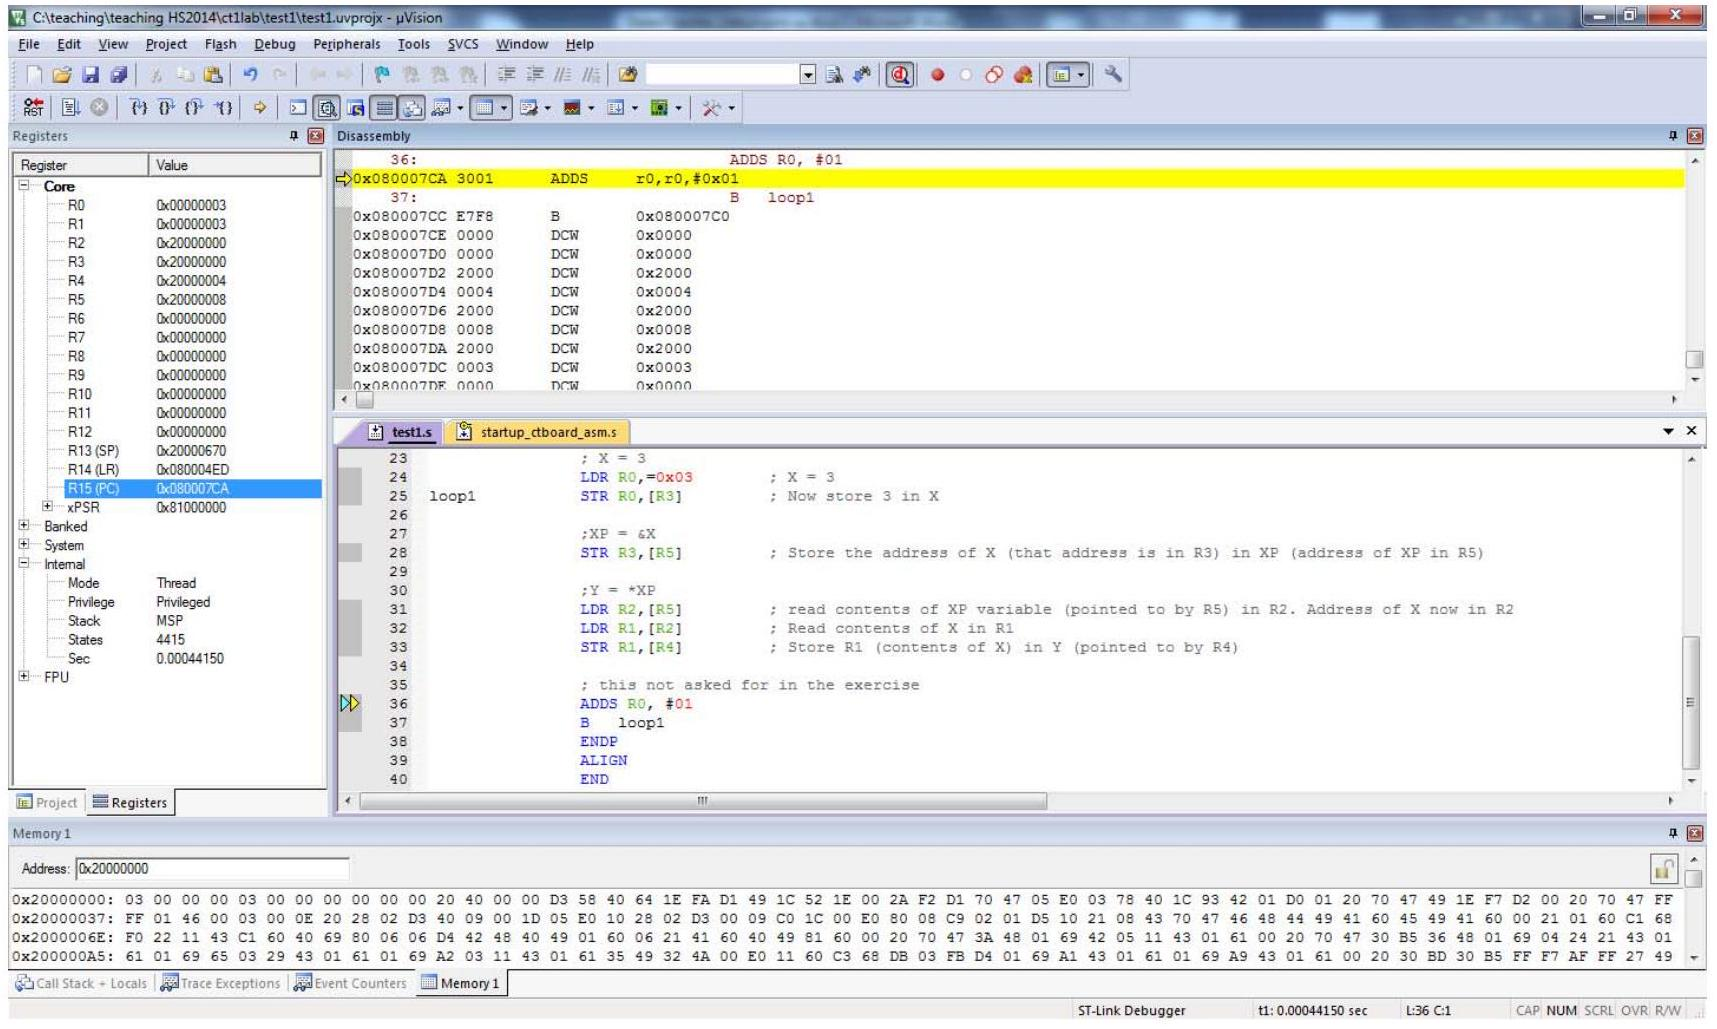
\includegraphics[width=\linewidth]{images/2025_01_02_eeffad754b73de6041b6g-10}

\begin{center}
\begin{tabular}{|c|c|c|c|c|c|}
\hline
19: & \multicolumn{2}{|r|}{LDR R3, = X} & 0x080007B8 4B05 & LDR & r3,[pc,\#20] ; @0x080007D0 \\
\hline
$20:$ & \multicolumn{2}{|r|}{LDR R4,=Y} & 0x080007BA 4C06 & LDR & r4,[pc,\#24] ; @0x080007D4 \\
\hline
21: & \multicolumn{2}{|r|}{LDR R5,=XP} & 0x080007BC 4D06 & LDR & r5,[pc,\#24] ; @0x080007D8 \\
\hline
22: &  &  &  &  &  \\
\hline
23: & \multicolumn{2}{|r|}{; $\mathrm{X}=3$} &  &  &  \\
\hline
24: & \multicolumn{2}{|r|}{LDR R0,=0x03} & 0x080007BE 4807 & LDR & r0,[pc,\#28] ; @0x080007DC \\
\hline
25: loop1 & \multicolumn{2}{|r|}{STR R0,[R3]} & 0x080007C0 6018 & STR & r0,[r3,\#0x00] \\
\hline
26: &  &  &  &  &  \\
\hline
27: & \multicolumn{2}{|r|}{; $\mathrm{XP}=$ \& X} &  &  &  \\
\hline
28: & \multicolumn{2}{|r|}{STR R3,[R5]} & 0x080007C2 602B & STR & r3,[r5,\#0x00] \\
\hline
29: &  &  &  &  &  \\
\hline
30: & \multicolumn{2}{|r|}{; $\mathrm{Y}=$ * XP} &  &  &  \\
\hline
31: & \multicolumn{2}{|r|}{LDR R2,[R5]} & 0x080007C4 682A & LDR & r2,[r5,\#0x00] \\
\hline
32: & \multicolumn{2}{|r|}{LDR R1,[R2]} & 0x080007C6 6811 & LDR & r1,[r2,\#0x00] \\
\hline
33: & \multicolumn{2}{|r|}{STR R1,[R4]} & 0x080007C8 6021 & STR & r1,[r4,\#0x00] \\
\hline
34: &  &  &  &  &  \\
\hline
35: & \multicolumn{3}{|r|}{; this not asked for in the exercise} &  &  \\
\hline
36: & \multicolumn{2}{|r|}{ADDS R0, \#01} & 0x080007CA 3001 & ADDS & r0,r0,\#0x01 \\
\hline
37: & B & loop1 & 0x080007CC E7F8 & B & 0x080007C0 \\
\hline
0x080007CE 0000 & DCW & $0 \times 0000$ &  &  &  \\
\hline
0x080007D0 0000 & DCW & $0 \times 0000$ &  &  &  \\
\hline
0x080007D2 2000 & DCW & $0 \times 2000$ &  &  &  \\
\hline
0x080007D4 0004 & DCW & $0 \times 0004$ &  &  &  \\
\hline
0x080007D6 2000 & DCW & $0 \times 2000$ &  &  &  \\
\hline
0x080007D8 0008 & DCW & $0 \times 0008$ &  &  &  \\
\hline
0x080007DA 2000 & DCW & $0 \times 2000$ &  &  &  \\
\hline
0x080007DC 0003 & DCW & $0 \times 0003$ &  &  &  \\
\hline
0x080007DE 0000 & DCW & $0 \times 0000$ &  &  &  \\
\hline
0x080007E0 0800 & DCW & $0 \times 0800$ &  &  &  \\
\hline
\end{tabular}
\end{center}

Another possible solution for exercise 9 a.\\
As given by the C compiler when code was written in C .\\
Note the MOVS. (This is not always good because it affects flags. So it should be used carefully)

\begin{verbatim}
This solution does not use pseudo instructions
It is here for you to see what the compiler could do
In a normal solution in assembler, it is better to use pseudo
instructions in order to create the literal pool. See solution
above.
The lines in blue are only there for help.
    x = 3;
0x08000254 2003 MOVS r0,#0x03
0x08000256 4905 LDR r1,[pc,#20] ; @0x0800026C
0x08000258 6008 STR r0,[r1,#0x00]
    xp = &x;
0x0800025A 4608 MOV r0,r1
0x0800025C 4904 LDR r1,[pc,#16] ; @0x08000270
0x0800025E 6008 STR r0,[r1,#0x00]
    y = *xp;
0x08000260 4608 MOV r0,r1
0x08000262 6800 LDR r0,[r0,#0x00]
0x08000264 6800 LDR r0,[r0,#0x00]
0x08000266 4903 LDR r1,[pc,#12] ; @0x08000274
\end{verbatim}

\end{comment}
